\documentclass{standalone}
\usepackage{tikz,pgfplots}
\pgfplotsset{compat=newest}
\begin{document}

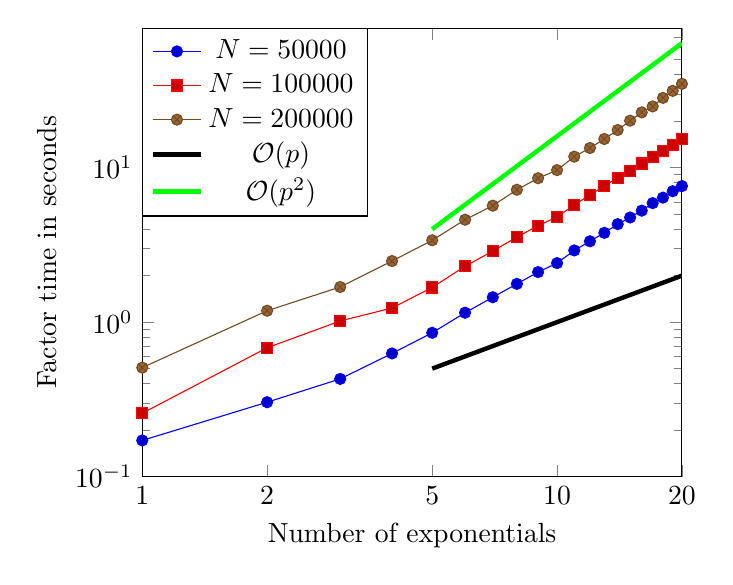
\begin{tikzpicture}
\begin{loglogaxis}[
	xlabel={Number of exponentials},
	ylabel={Factor time in seconds},
	xmin=1, xmax=20,
	ymin=1e-1, ymax=80,
%	log x ticks with fixed point,
	xticklabel style={/pgf/number format/.cd,fixed,precision=2},
    xticklabel={%
      \pgfmathfloatparsenumber{\tick}%
      \pgfmathfloatexp{\pgfmathresult}%
      \pgfmathprintnumber{\pgfmathresult}%
	  },
	  xtick={1, 2, 5,  10, 20},
	  legend style={
	  	at={(0.0,1.0)},
		anchor=north west},
%	xticklabel=\pgfmathparse{10^\tick}\pgfmathprintnumber{\pgfmathresult}
]
%Fast N=50000
\addplot
coordinates{
(1, 0.171438) (2, 0.302995) (3, 0.428946) (4, 0.627026) (5, 0.852955) (6, 1.15047) (7, 1.44919) (8, 1.76902) (9, 2.109) (10, 2.41092) (11, 2.9131) (12, 3.33818) (13, 3.78692) (14, 4.3096) (15, 4.76071) (16, 5.27168) (17, 5.89564) (18, 6.40062) (19, 7.0439) (20, 7.60488) 
};
\addlegendentry{$N=50000$}
%Fast N=100000
\addplot
coordinates{
(1, 0.257065) (2, 0.682426) (3, 1.01703) (4, 1.23474) (5, 1.67739) (6, 2.29856) (7, 2.88753) (8, 3.549) (9, 4.21465) (10, 4.79732) (11, 5.73575) (12, 6.66259) (13, 7.61323) (14, 8.60503) (15, 9.54356) (16, 10.6329) (17, 11.7085) (18, 12.8122) (19, 13.9846) (20, 15.3897) 
};
\addlegendentry{$N=100000$}
%Fast N=200000
\addplot
coordinates{
(1, 0.507383) (2, 1.18534) (3, 1.68866) (4, 2.48588) (5, 3.38777) (6, 4.60491) (7, 5.67833) (8, 7.19703) (9, 8.54981) (10, 9.64664) (11, 11.7903) (12, 13.411) (13, 15.3421) (14, 17.5406) (15, 20.1635) (16, 22.8149) (17, 24.9367) (18, 28.3087) (19, 31.4349) (20, 34.9056) 
};
\addlegendentry{$N=200000$}
%O(p) scaling
\addplot[ultra thick, no marks]
coordinates{
(5, 0.5) (20, 2)
};
\addlegendentry{$\mathcal{O}(p)$}
%O(p2) scaling
\addplot[green, ultra thick, no marks]
coordinates{
(5, 4) (20, 64)
};
\addlegendentry{$\mathcal{O}(p^{2})$}
\end{loglogaxis}
\end{tikzpicture}
\end{document}